% !TeX spellcheck=eng

\chapter{The Dataset}
The dataset provided contains information about forest cover types. It contains seven typologies of forests labeled from $1$ to $7$, fiftyfour features listed in \autoref{tab:fetaures} along with an identification number and a column which contains the label associated to the record.
\begin{table}[htpb]
	\centering
\begin{tabular}{|c|c|}
	\hline 
	\textbf{Name} & \textbf{Measurement} \\ 
	\hline 
	Elevation & meters \\ 
	\hline 
	Aspect & azimuth \\ 
	\hline 
	Slope & degrees \\ 
	\hline 
	Horizontal distance to hydrology & meters \\ 
	\hline 
	Vertical distance to hydrology & meters \\ 
	\hline 
	Horizontal distance to roadways & meters \\ 
	\hline 
	Hillshade 9am & $[0..255]$ \\ 
	\hline 
	Hillshade noon & $[0..255]$ \\ 
	\hline 
	Hillshade 3pm & $[0..255]$ \\ 
	\hline 
	Horizontal distance to fire points & meters \\ 
	\hline 
	Wilderness area & $\lbrace0, 1\rbrace$ \\ 
	\hline 
	Soil type & $\lbrace0, 1\rbrace$ \\ 
	\hline 
\end{tabular}
\caption{Table of the features provided by the dataset. The ``Wilderness area'' feature is divided in four binary columns one for each area studied, as for the ``Soil type'' feature which is divided in fourty binary columns.}
\label{tab:fetaures}
\end{table}
\begin{figure}[htpb]
	\centering
	\begin{tabular}{cc}
		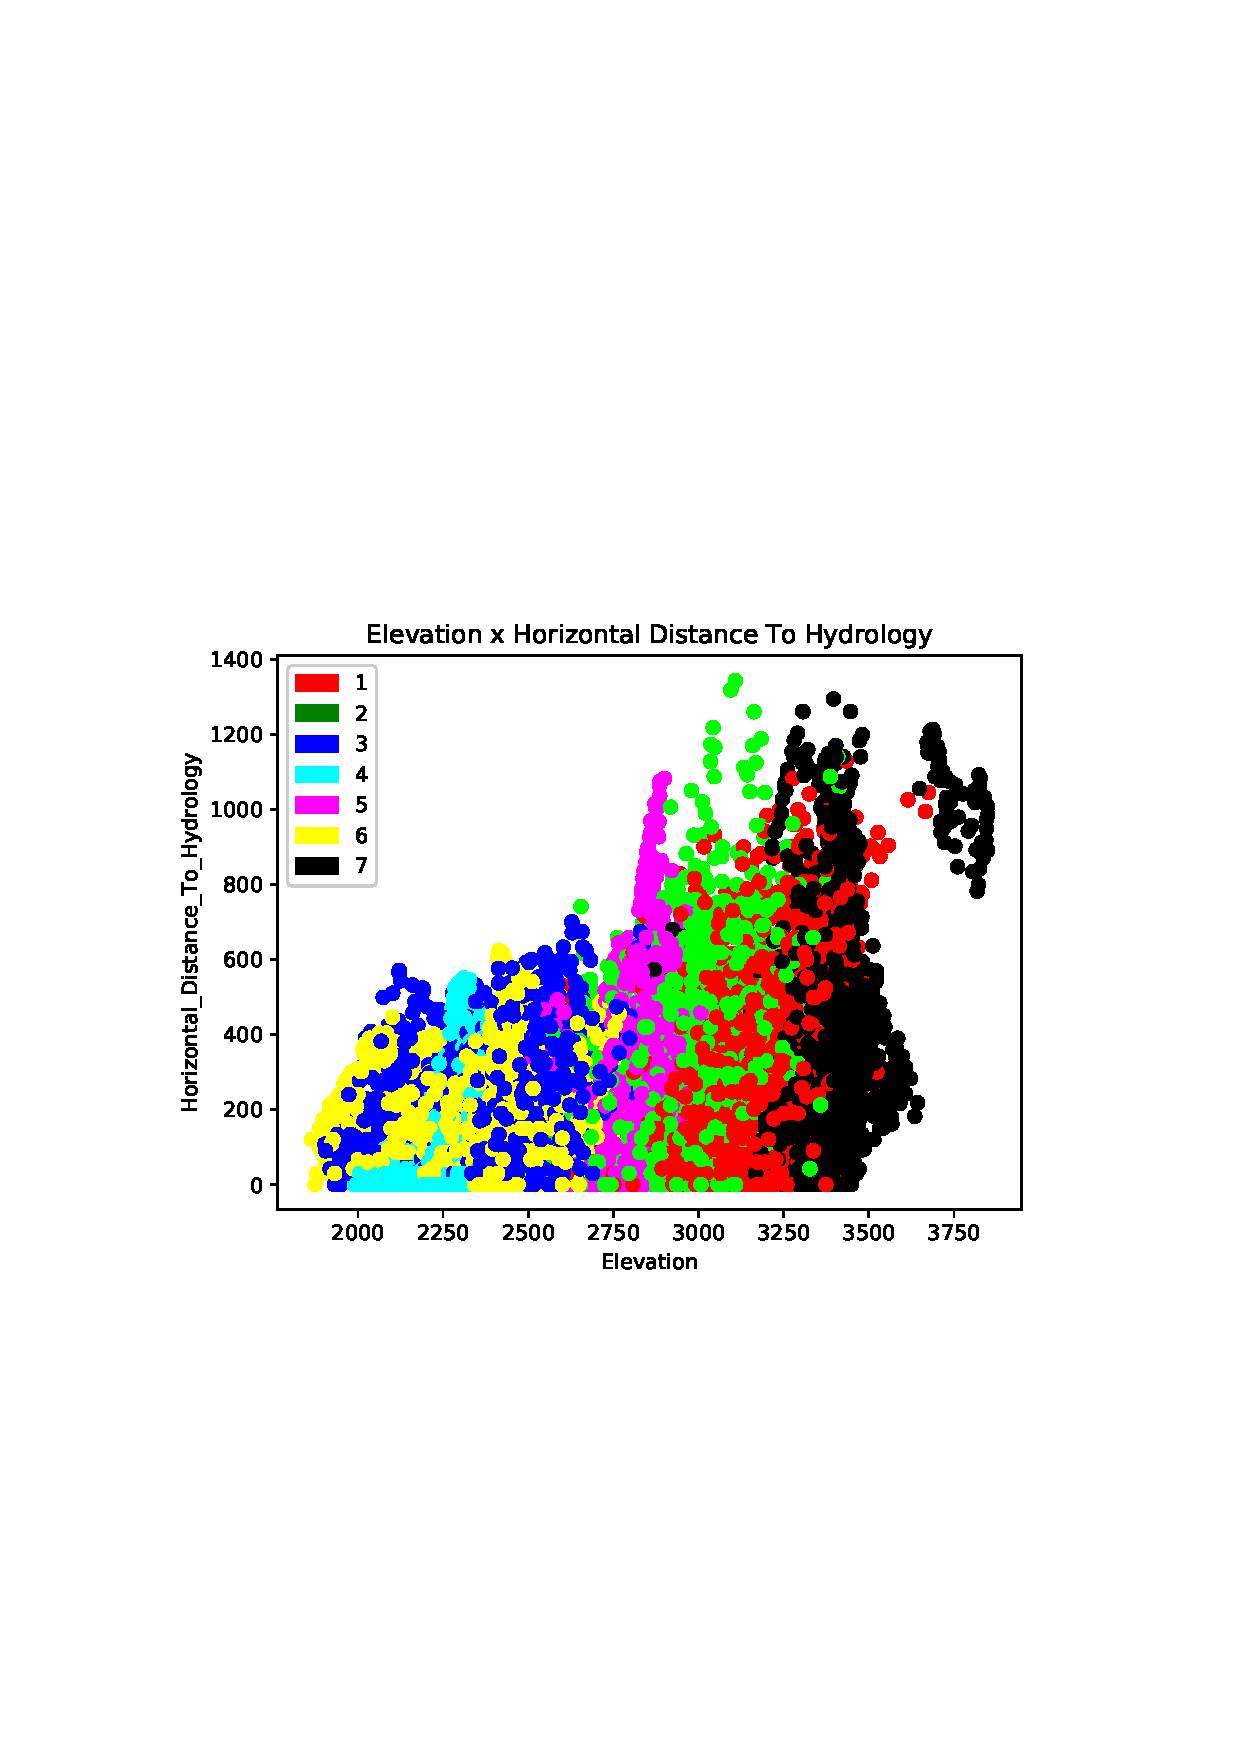
\includegraphics[scale=0.45]{figs/1.pdf}	& 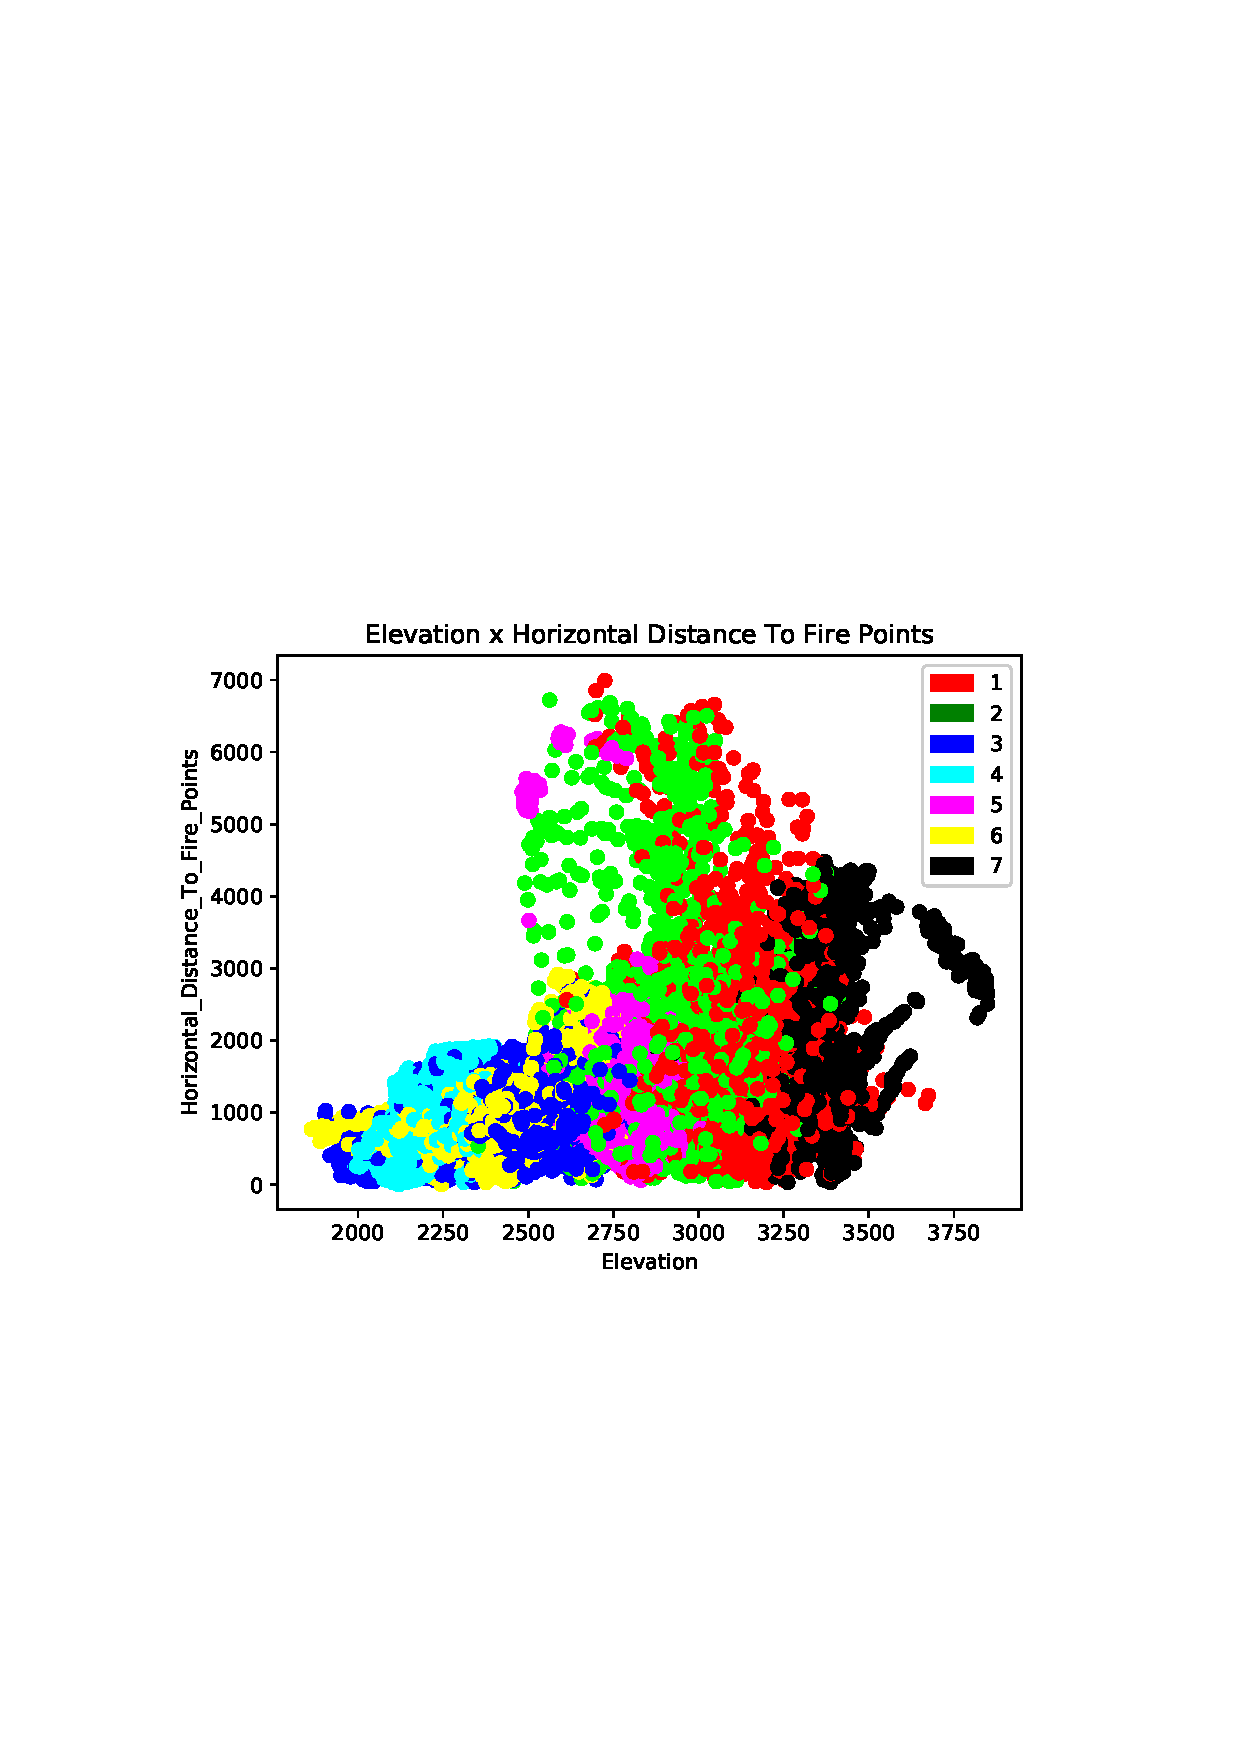
\includegraphics[scale=0.45]{figs/2.pdf}\\ 
		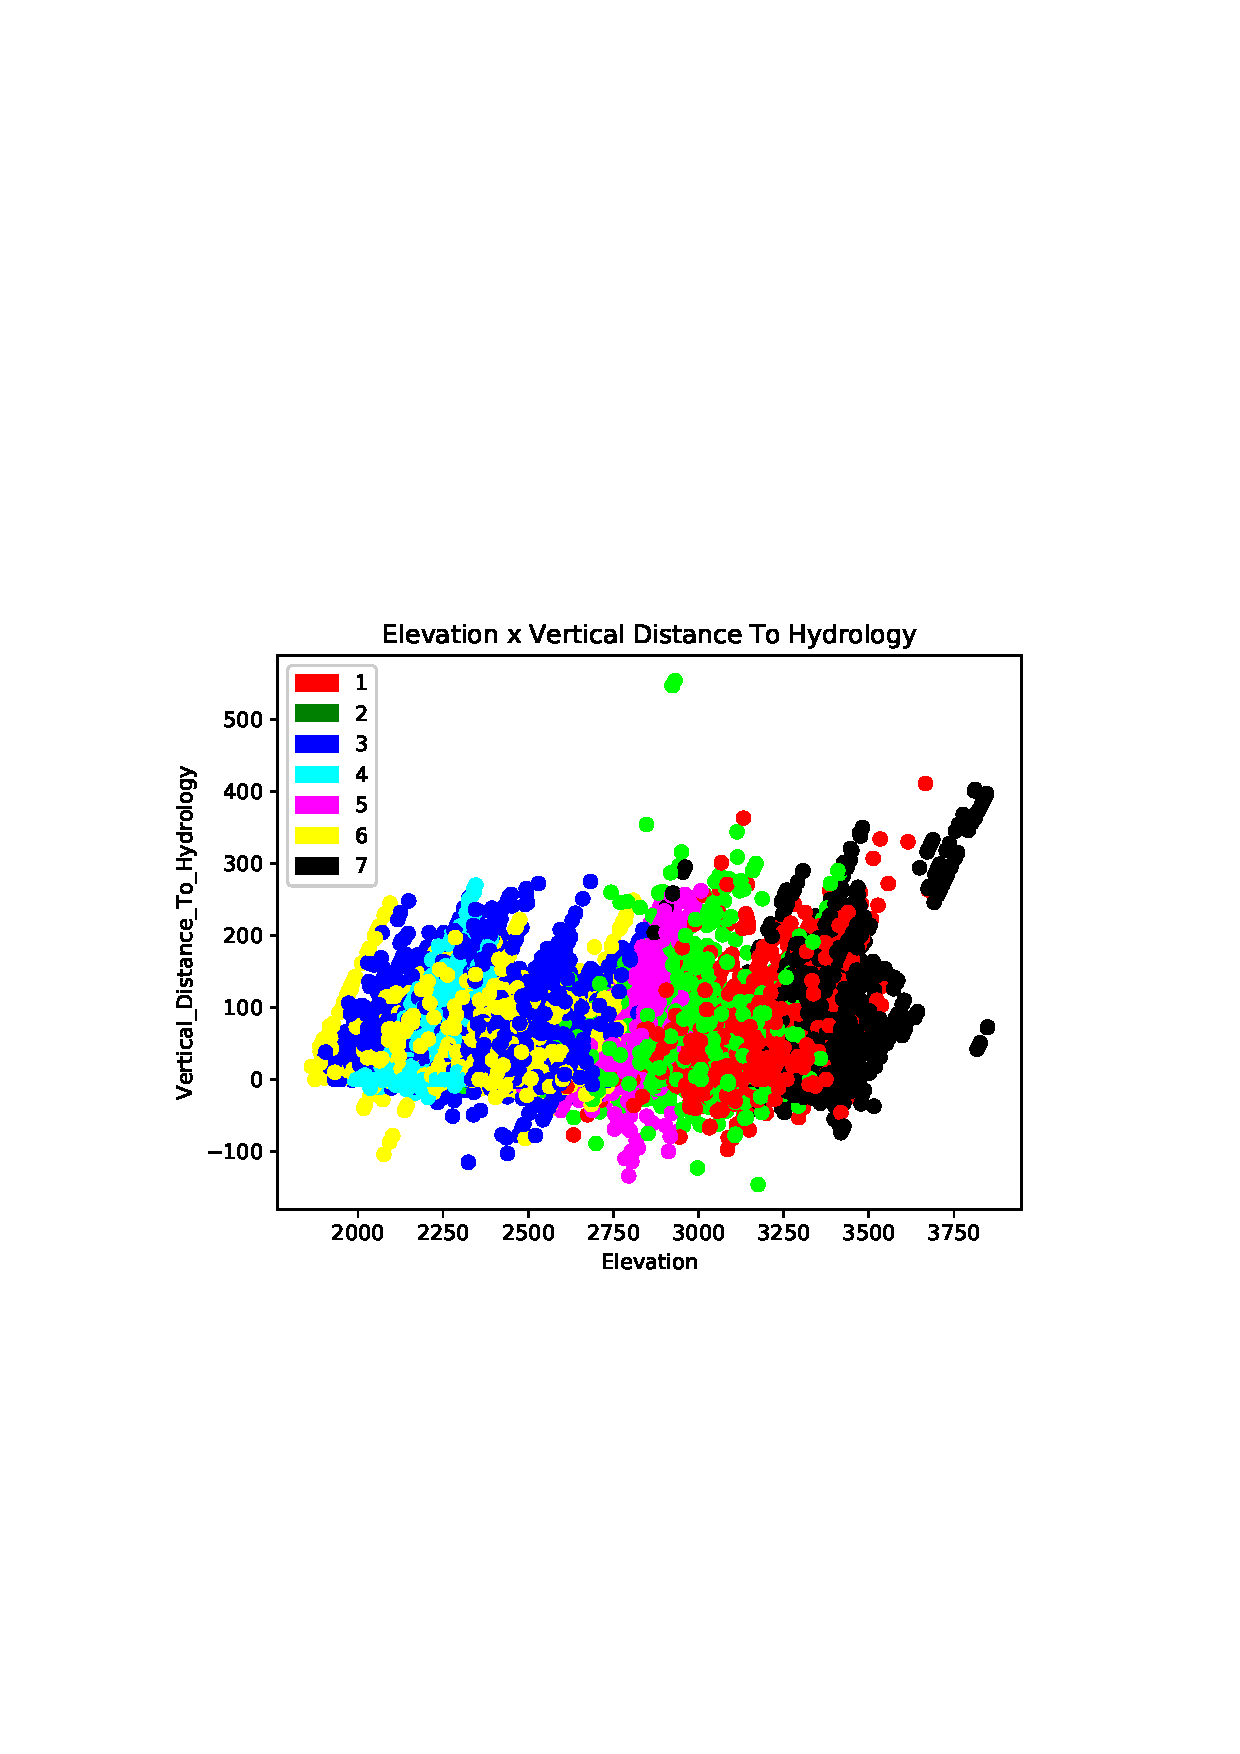
\includegraphics[scale=0.45]{figs/3.pdf} & 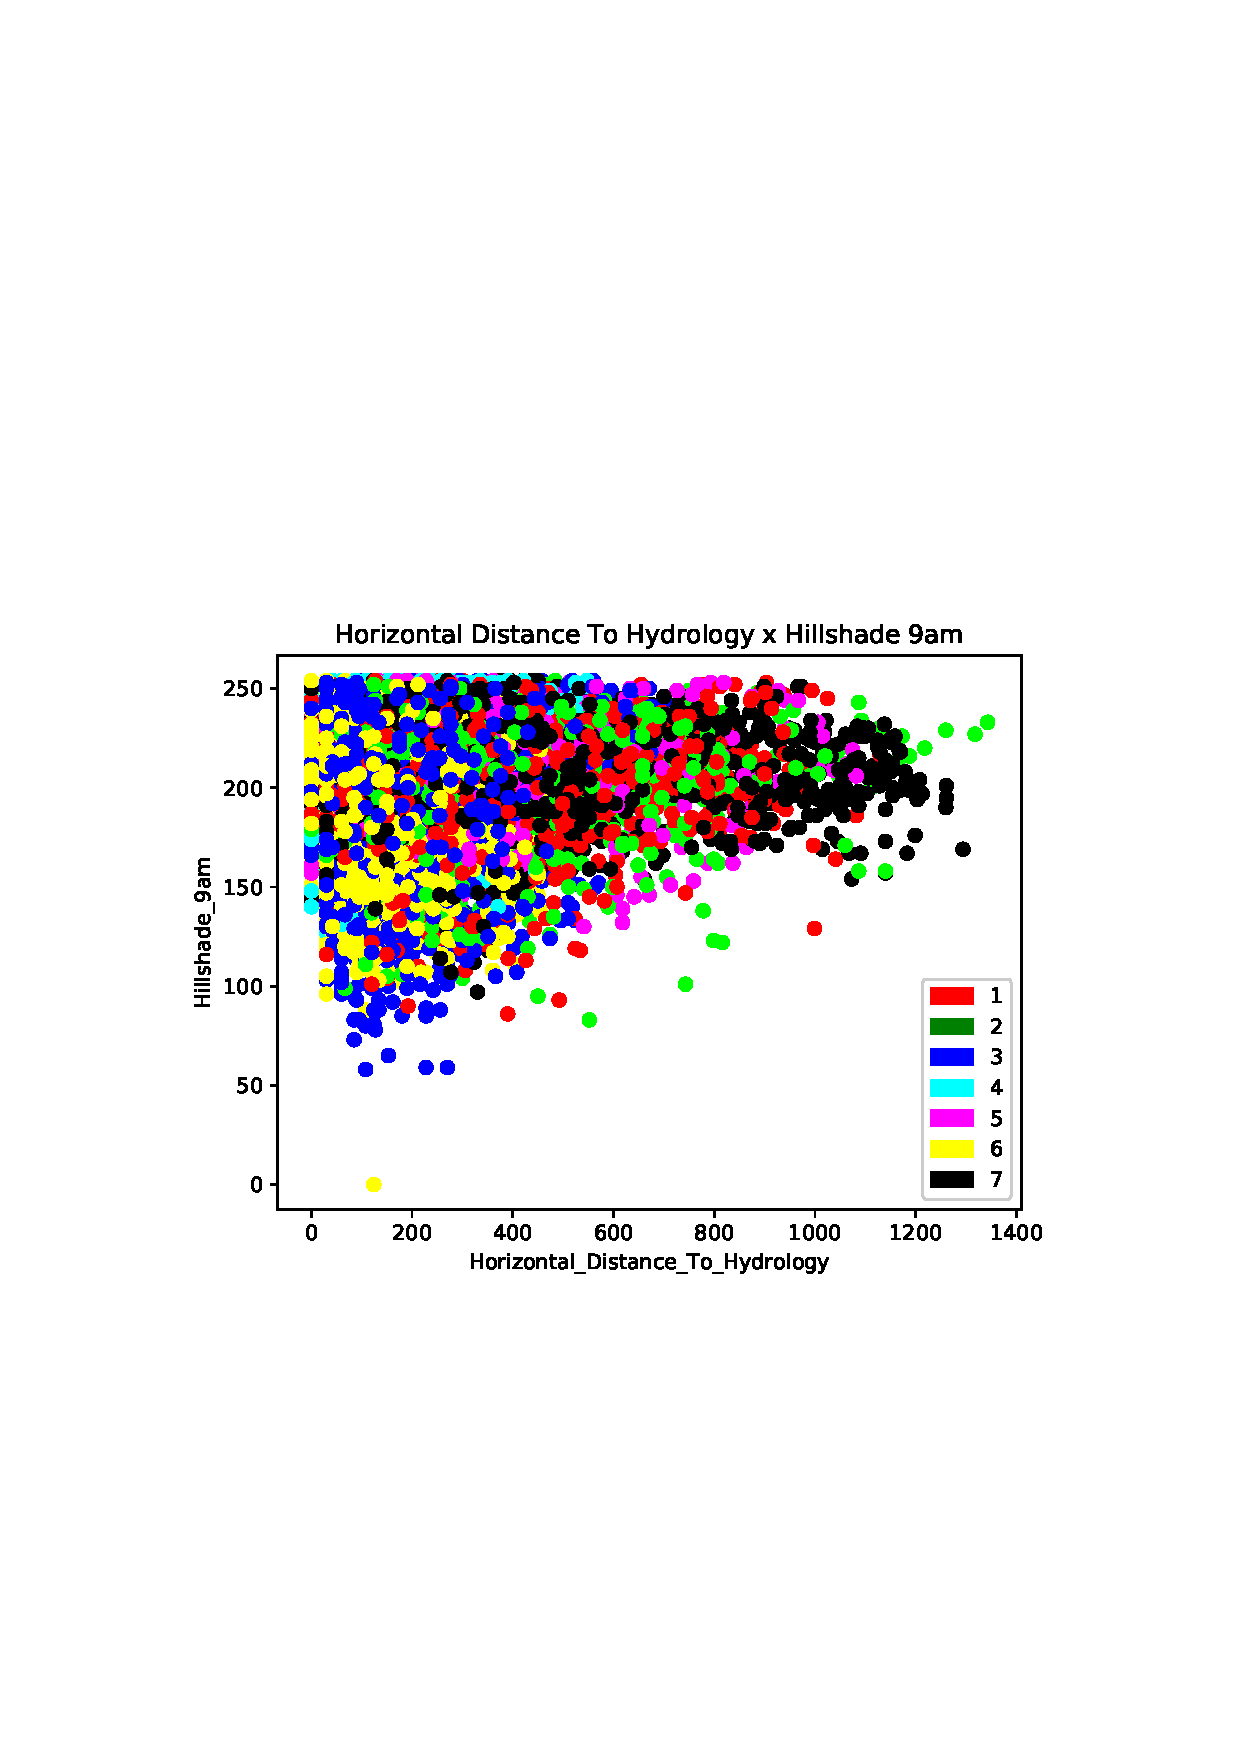
\includegraphics[scale=0.45]{figs/4.pdf} \\ 
	\end{tabular} 
	\caption{Four examples of labeled record}
	\label{fig:plots}
\end{figure}
In \figurename~\ref{fig:plots} we provide four examples of labeling based only by two feature per plot. In the first row and in the first plot of the second row, the labels are well ``separated'', suggesting that some of those features could be a strong candidate for classification. The last plot, located in the bottom\-right of the image, do not separate well the seven labels, suggesting that the Horiontal distance to hydrology combined (only) with the Hillshade 9am features are not good features in order to classify with a low statistical risk.